\section{Erstellen der Doubly-connected Edge List}
\subsection{Graph Klasse}
Die zweidimensionalen Operationen der Anwendung werden von der \icode{Graph}-Klasse durchgeführt. 
Übergibt man dieser eine Liste aus Linien, welche jeweils aus einem Start- und Endortsvektor bestehen, wird auf diesen basierend eine DCEL berechnet.
Dafür werden die drei graphischen Elemente der Typen \icode{Edge}(Kante), \icode{Node}(Knoten) und \icode{Face}(Fläche) gespeichert.

\subsection{Verarbeitung der Linien}
Beginnend werden gleichzeitig die Knoten und Kanten der zu generierenden DCEL erstellt.
\subsection{Vector-to-Node Konvertierung}
Aus einem Ortsvektor kann die Funktion \icode{createNode()} einen kongruenten Knoten mit gleichen Ursprungskoordinaten, aber ohne Referenz auf eine anliegende Kante, erstellen. 
Desweiteren wird, falls ein Knoten zu einem abgefragten Punkt schon generiert wurde, dieser zurückgeben.
\begin{code}[\icode{createNode()} Funktion]
	private Node createNode(Vector p) {
		for (Node n : nodes) {
			if (n.getOrigin().equals(p)) {
				return n;
			}
		}
		nodes.add(new Node(p));
		return (nodes.get(nodes.size() - 1));
	}
\end{code}
\subsection{Line-to-Edge Konvertierung}
\label{subsec:ltoe} 
Die \icode{processData} Funktion greift auf \icode{createNode()} zu und erstellt die Liste aus Kanten mit den jeweiligen Start- und Endknoten.
Auch hier gibt es noch keine abgespeicherten Zusammenhänge zwischen den einzelnen Kanten.
\begin{code}[Line-to-Edge Konvertierung]
private void processData(ArrayList<Line> ls) {
	for (Line l : ls) {
		edges.add(new Edge(createNode(l.getP1()), createNode(l.getP2())));
	}
}
\end{code}
Basierend auf dieser Grundlage müssen alle folgenden Kalkulationen der \icode{Graph}-Klasse durchgeführt werden.
\subsection{Zwillingskantengenerierung}
Durch Vertauschen der Start- und Endknoten wird nun für jede existente Kante eine entgegengesetzt-laufende komplementäre \q{Zwillingskante} gebildet.
In der Anwendung wird so die Liste der Kanten um ihre Größe erweitert.
Direkt nach dem Hinzufügen der Zwillingskante wird jeweils eine Referenz erstellt, welche beide Zwillinge miteinander verknüpft. 
Durch die Zwillingskanten werden folgende Operationen in der DCEL vereinfacht, da jede Fläche nun von einer eindeutigen Menge an Kanten begrenzt ist und ein Umlaufsinn dieser festgestellt werden kann.

\subsection{Nachfolger- und Vorgängerermittlung}
Für die Erstellung der Nachfolger- und Vorgängerreferenzen zwischen den Kanten, werden alle ausgehenden Kanten $E$ eines Knotens $N_i$ betrachtet.
Anschließend sortiert die Anwendung diese mittels der \icode{angle()}-Methode anhand des Winkels.
Dabei wird die jeweilige Kante $E_i$ in einen Vektor, welcher zwischen die beiden Kantenknoten gespannt werden kann, konvertiert, damit die \icode{angle()}-Funktion aufrufbar ist.
Diese gibt den Winkel des Vektors zur x-Achse im Intervall $(-\pi,\pi]$ aus.
Aus den angeordneten Kanten $E$ lassen sich unter Beachtung des mathematisch positivem Umlaufsinnes der Kanten an den Flächen nun folgende Beziehungen ableiten. 
\begin{enumerate}
	\item Die Zwillingskante von $E_{i+1}$ ist der Vorgänger von $E_i$
	\item $E_{i-1}$ ist der Nachfolger der Zwillingskante von $E_i$ 
\end{enumerate}
\begin{Bild}{Veranschaulichung 1. und 2.}
	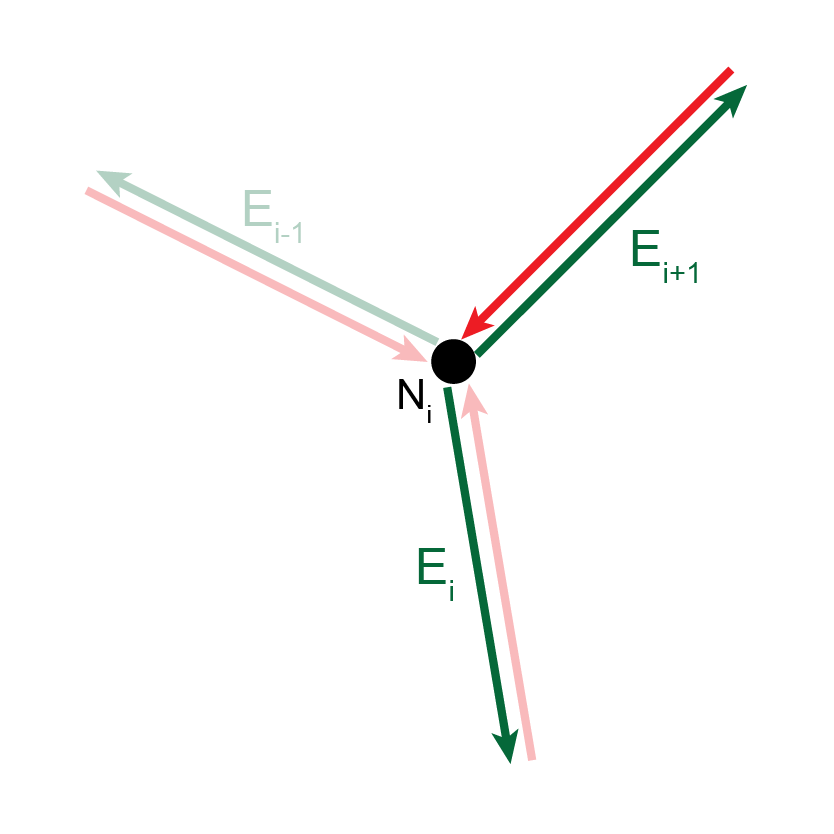
\includegraphics[width = 70mm]{Bilder/Beziehung1Kanten}
		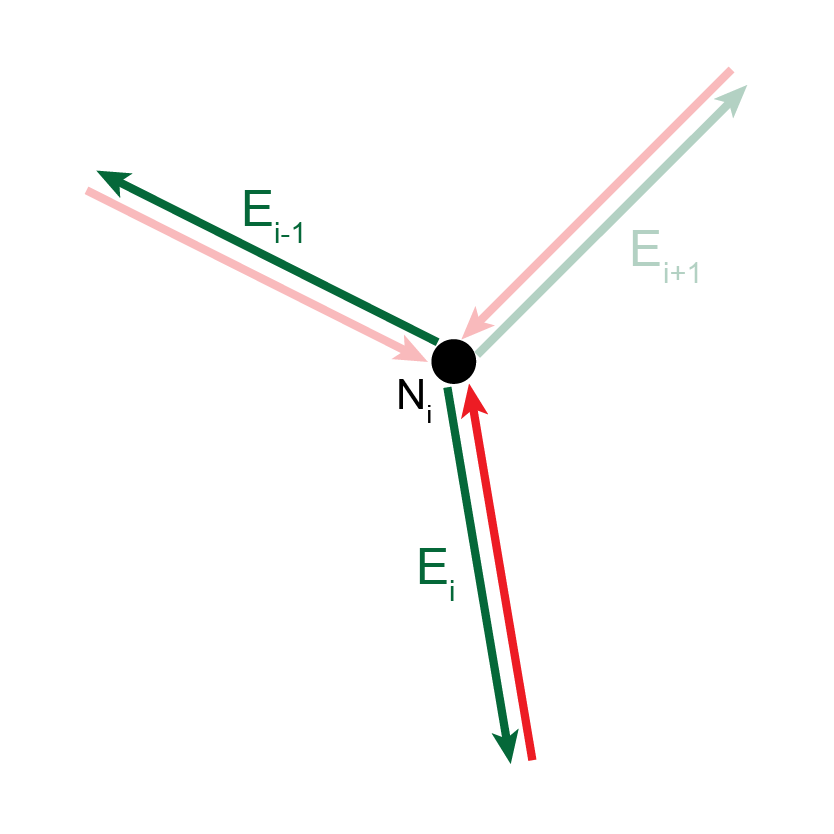
\includegraphics[width = 70mm]{Bilder/Beziehung2Kanten}
\end{Bild}
Falls $i-1$ bzw. $i+1$ die Indices der Menge $E$ mit $n$ Elementen überschreiten, wird anstattdessen $E_n$ bzw. $E_0$ gewählt. \\
Der aufgeführte Algorithmus wird für alle Knoten $N$ der DCEL fortgeführt, sodass alle Referenzen zwischen den Kanten fertiggestellt werden. 
\todoinline{code eventuell bilder definitiv}

\subsection{Flächenerstellung}
Mithilfe einer Schleife können die einzelnen Flächen erschlossen werden.
Es muss lediglich fortlaufend alle Nachfolger einer gewählten Kante gesucht werden bis die gefundene Kante einen Nachfolger darstellt, bis alle Kanten genau einmal behandelt wurden.
Dafür wurde eine repräsentative \icode{Boolean-ArrayList} mit der Länge der Kantenliste erstellt, die mit ihren Werten den Status der Kanten darstellt.
Folglich besteht diese am Anfang nur aus \icode{false} Werten die während der Schleife alle auf \icode{true} gesetzt werden.
Die Speicherung der Flächen folgt dem DCEL-Standard, sodass nur eine anliegende Kante zugewiesen wird, mit der man, aufgrund von den Referenzen alle Kanten und Knoten der Fläche ermitteln kann.
Das äußere Gebiet des planaren Graphen lässt sich an der Umlaufrichtung der Kanten erkennen.
Es ist die einzige Fläche, die im mathematisch negativen Drehsinn ausgerichtet ist.
Unterschieden wird sie im weiteren Programmablauf mithilfe der Gaußschen Trapezformel.
Bei negativer Umlaufrichtung ist das Ergebnis dieser negativ.\\
\todoinline{Bitte noch mal überarbeiten, total wirr}

\subsection{Vervollständigung der Knoten}
Die letzte nötige Operation ist die Speicherung einer anliegenden Edge in den Nodes.\\
\todoinline{man könnte das im code auch vorher tun denke ich}